\documentclass[aps,prd,preprintnumbers,nofootinbibn,twocolumn]{revtex4}
%showpacs,superscriptaddress,groupedaddress
\usepackage{graphicx}  % needed for figures
\usepackage{dcolumn}   % needed for some tables
\usepackage{bm}        % for math
\usepackage{amssymb}   % for math
\usepackage[utf8]{inputenc}
%\usepackage[spanish]{babel}
\usepackage{hyperref}

\usepackage{amsmath}
\usepackage{array}
\usepackage{appendix}
\usepackage{epsfig}
\usepackage{siunitx}
\usepackage{verbatim}
\hyphenation{arXiv}

\addtolength{\textheight}{1.6cm}

\newcommand{\dif}{\mathrm{d}}
\newcommand{\expo}[1]{\mathrm{e}^{#1}}
\newcommand{\tr}{\mathrm{tr}}
\newcommand{\sla}[1]{\!\not\!#1\,}

\makeatletter
\def\l@subsection#1#2{}
\def\l@subsubsection#1#2{}
\makeatother
\begin{document}


\title{NEW APPLICATIONS OF THE COLEMAN-WEINBERG MODEL\\[0.4cm]}
\thispagestyle{empty}


\date{de 2016}


\begin{abstract}
\begin{center}
\vspace{0.7cm}

{\bf Autor:}\\

\vspace{0.2cm}

Jorge Alda Gallo $^{(1)}$\\

\vspace{1cm}

{\bf Director:}\\

\vspace{0.2cm}

J. A. R. Cembranos $^{(2)}$\\

\vspace{0.6cm}


\vspace{5cm}
\begin{center}

\includegraphics[width=0.30\textwidth]{ucmlogo}
\end{center}
\vspace{5cm}
\end{center}

$^{(1)}$  E-mail: \href{mailto:jalda@ucm.es}{jalda@ucm.es}

$^{(2)}$ E-mail: \href{mailto:cembra@fis.ucm.es}{cembra@fis.ucm.es}
\vspace{8cm}

\end{abstract}




\clearpage


\maketitle

\begin{widetext}
\begin{quotation}

{\bf Resumen:}\\



\vspace{2cm}

{\bf Abstract:}\\



\vspace{2cm}
\end{quotation}
\end{widetext}
\tableofcontents


\vspace{5cm}




\newpage
\clearpage

\section{Introduction}
Our current understanding of the non-gravitational interactions, the Standard Model (SM) of particle physics, is based on a gauge chiral symmetry group $\mathsf{SU}(3)_C \times \mathsf{SU}(2)_L \times \mathsf{U}(1)_Y $. But this is at odds with both massive fermions and massive gauge bosons. Thus, there seemed to be a big problem, since fermions and the W and Z bosons are experimentally observed to have mass. The solution was devised by Higgs, Brout, Englert, Guralnik, Hagen and Kibble (working on a previous concept by Anderson), called the Higgs mechanism. They proposed the existence of a scalar field charged under $\mathsf{SU}(2)_L \times \mathsf{U}(1)_Y$, the Higgs field, with a potential with degenerated vacua, wich breaks said symmetry. The coupling with the generators of $\mathsf{SU}(2)_L \times \mathsf{U}(1)_Y$ is responsible for the masses of the W and Z bosons in the broken phase, and Yukawa couplings with quarks and leptons cause their masses. 


According to the SM, the Higgs field $H$ is characterized by the following potential
\begin{equation}\label{eq:HiggsPotential}
V = m^2 H^\dagger H + \lambda_h (H^\dagger H)^2\ .
\end{equation}

Here, $m^2 < 0$, which means that $H=0$ is unstable. Thus, the Higgs field has a vacuum expectation value (vev) $v_h=\SI{246.2}{\giga\electronvolt}$ (known from masses of the $W$ and $Z$ bosons and muon decay, \cite{Agashe:2014kda}). This causes an spontaneous symmetry breaking that provides the masses for fermions and gauge bosons. The condition for the minimum of the potential is 
\begin{equation}
m^2 = -2\lambda_h v_h^2\ .
\end{equation}

The physical mass of the Higgs boson is determined as the value of the second derivative of the potential at the vacuum, that is, 
\begin{equation}
m_h^2 = 2 \lambda_h v_h^2=-m^2\ .
\end{equation}

The Higgs boson, the excitation of the Higgs field, has remained for a long time the elusive last piece of the SM to be discovered. The waiting came to an end on 2012, when it was announced the discovery at LHC \cite{Aad:2012tfa,Chatrchyan:2012xdj} of a new resonance at \SI{125}{\giga\electronvolt}. But a \SI{125}{\giga\electronvolt} SM Higgs boson leaves some open questions: vacuum metastability and hierarchy problem.
 
Quantum corrections to the Higgs potential are controlled by the Yukawa coupling of the top quark. The current value of this coupling might mean that $\lambda_h$ turns negative. Thus, the electroweak vacuum would be metastable \cite{EliasMiro:2011aa}, and it would be able to decay to a lower energy vacuum.

The quadratic term in the Higgs potential is the only dimesionful parameter in the SM. Naturalness indicates that the Higgs mass should be similar to the other energy scale in any relativistic quantum field theory, the Planck scale. But the Higgs mass and the Planck energy are quite different, in fact they are 17 orders of magnitude apart, which leads to the so-called hierarchy problem \cite{Iso:2013aqa}. 

An alternative proposal for the origin of the Higgs boson mass is due to Coleman and Weinberg \cite{Coleman:1973jx} (CW). In this model, quadratic term is set to zero, and the physical Higgs mass is generated by radiative corrections to the quartic term in a process called dimensional transmutation. In this way, the CW lagrangian is classically scale invariant and is free of the hierarchy problem. The large hierarchy between the Planck and the Higgs scales is exponentially controlled by the running of the quartic coupling. 

The CW classical potential is
\begin{equation}
V_{CW}^{(0)} = \lambda_h (H^\dagger H)^2\ .
\end{equation}

In the quantum realm $\lambda_h$ is no longer a constant, but depends on the energy scale - that can be identified with the vev $v_h$. In the one-loop approximation, the dependence is 
\begin{equation}
\lambda(v_h) \approx \beta_h \ln\left(\frac{v_h}{M}\right)\ , 
\end{equation}
where $M$ is an arbitrary parameter with dimensions of mass. The one-loop CW potential is now

\begin{equation}
V_{CW}^{(1)} \approx \beta_h v_h^4 \ln \left(\frac{v_h}{M}\right)\ .
\end{equation}

The classical potential only has a minimum at the origin, and therefore the vacuum state doesn't break the electroweak symmetry. But the radiative corrections move this minimum to 
\begin{equation}
v_h = \mathrm{e}^{-1/4} M\ ,
\end{equation}
which is a stable minimum, this is, the curvature at the extremum is $m_h^2 > 0$. The comparison between the classical and the one-loop CW potential is shown in \textsc{fig.} \ref{fig:CWpotential}

\begin{figure}[b]
\centering
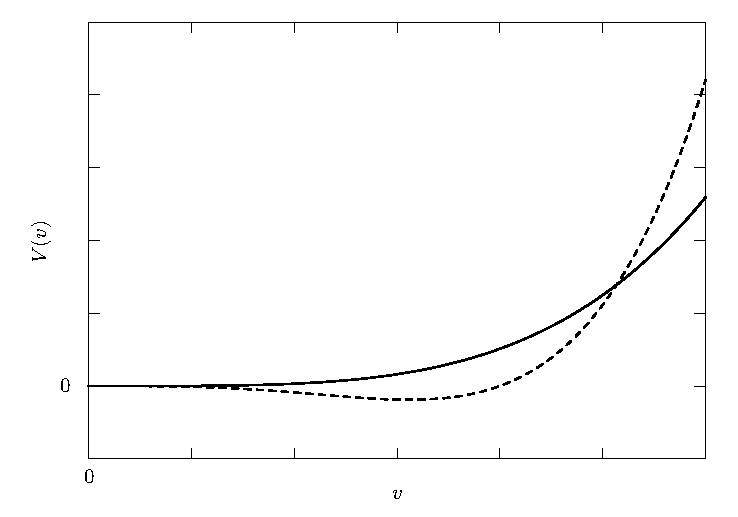
\includegraphics[width=\columnwidth]{potential}
\caption{Solid line: classical Coleman-Weinberg potential. Dashed line: one-loop Coleman-Weinberg potential.}\label{fig:CWpotential}
\end{figure} 

Unfortunately, in the SM this running is dominated by the top Yukawa coupling, and the predicted value for the Higgs mass is far too low.  

In the last few years, the CW mechanism has regained popularity, and some modifications have been proposed \cite{Dermisek:2013pta, Hill:2014mqa, Antipin:2015kgh}. We will study a model where the CW is not realized by the Higgs boson itself, but by an additional scalar boson coupled to it. In the context of dark matter and inflation, such models are called \textit{portal Higgs} \cite{Patt:2006fw, Englert:2013gz}, and the new scalar field is usually either a singlet or a $\mathsf{SU}(2)$ doublet. We will consider a scalar field charged under a more general $\mathsf{SU}(N_S)$ symmetry.

This document is organized as follows: In section \ref{sect:model} we present this model. In section \ref{sect:RG} we examine the Renormalization Group flow of the coupling constants and the conditions required by the renormalizability of the model. In section \ref{sec:mixing} we study whether the Higgs field and the new field mix to form mass eigenstates. In section \ref{sec:GUT} we focus in the behavior of the couplings in the Grand Unification Theory (GUT) energy scale.

\section{The model} \label{sect:model}
In our model, the Higgs $H$ is a massless scalar boson in the fundamental representation of $\mathsf{SU}(2)$. In addition, we have another massless scalar field $S$ in the fundamental representation of a $\mathsf{SU}(N_S)$ gauge symmetry. Their potential is
\begin{equation}\label{eq:CWpotential}
V = \lambda_h (H^\dagger H)^2 + \lambda_{hs} (H^\dagger H) (S^\dagger S) + \lambda_s (S^\dagger S)^2\ .
\end{equation}

The model has three different phases: at large energies, both the $\mathsf{SU}(N_S)$ and the  $\mathsf{SU}(2)_L \times \mathsf{U}(1)_Y$ symmetries remain unbroken. When the energy scale gets lower, the scalar $S$ breaks the $\mathsf{SU}(N_S)$ symmetry a la Coleman-Weinberg, and the Higgs potential acquires its SM form. Finally, at low energies the electroweak symmetry gets broken and all particles get their masses as usual.

We expand the field $S$ around its vev $v_s$, $|S| = v_s + \frac{\sigma}{\sqrt{2}}$. The couplings depend on the physical field $\sigma$ according to $\lambda(|S|) = \beta \log(|S|/M)$:
\begin{subequations}
\begin{align}
\lambda_h\left(v_s + \frac{\sigma}{\sqrt{2}}\right) &\approx \lambda_h(v_s) + \beta_h \left(\frac{\sigma}{\sqrt{2}v_s}-\frac{\sigma^2}{4 v_s^2}\right)\ ,\\
\lambda_s\left(v_s + \frac{\sigma}{\sqrt{2}}\right) &\approx \lambda_s(v_s) + \beta_h \left(\frac{\sigma}{\sqrt{2}v_s}-\frac{\sigma^2}{4 v_s^2}\right)\ ,\\
\lambda_{hs}\left(v_s + \frac{\sigma}{\sqrt{2}}\right) &\approx \lambda_{hs}(v_s) + \beta_{hs} \left(\frac{\sigma}{\sqrt{2}v_s}-\frac{\sigma^2}{4 v_s^2}\right)\ .
\end{align}
\end{subequations}

The condition for the minimum of the potential is:
\begin{equation}
\frac{\dif V_\mathrm{eff}}{\dif \sigma}\Big|_{\substack{\sigma=0\\ H=0}} = \frac{v_s^3}{\sqrt{2}}(4\lambda_s + \beta_s) = 0\ ,  \qquad 4\lambda_s = - \beta_s \ . 
\end{equation}

The mass of the scalar is now given by
\begin{equation}
m_s^2 = \frac{\dif^2 V_\mathrm{eff}}{\dif \sigma^2}\Big|_{\substack{\sigma=0\\ H=0}} \! =\frac{v_s^2}{2} (12 \lambda_s +7\beta_s) =2\beta_s v_s^2 = -8 \lambda_s v_s^2\ ,
\end{equation}
where we learn that $\beta_s > 0 $ and $ \lambda_s < 0$. We now can rewrite \textsc{Eq.}\ \eqref{eq:CWpotential} as
\begin{equation}
V_\mathrm{eff} = V_H (H) + V_S (\sigma) + V_\mathrm{int}(H, \sigma)\ ,
\end{equation}
with
\begin{subequations}
\begin{align}
V_H =& m^2 H^\dagger H + \lambda_h (H^\dagger H)^2\label{eq:quadraticCW}\ , \\
V_S =& \frac{1}{2}m_s^2 \sigma^2 + \sqrt{2}(\lambda_s+\beta_s)v_s \sigma^3 + \frac{\lambda_s+\beta_s}{4}\sigma^4 \nonumber \\ &- \frac{\beta_s}{2^{5/2} v_s}\sigma^5 - \frac{\beta_s}{16 v_s^2}\sigma^6\ \label{eq:Spotential},\\
V_\mathrm{int} =& \frac{(2\lambda_{hs} + \beta_{hs})v_s}{\sqrt{2}}\sigma H^\dagger H + \frac{2\lambda_{hs} + 3\beta_{hs}}{4}\sigma^2 H^\dagger H\nonumber\\ &+ \frac{\beta_h}{\sqrt{2} v_s}\sigma (H^\dagger H)^2 - \frac{\beta_{hs}}{8 v_s^2}\sigma^4 H^\dagger H\nonumber \\ &- \frac{\beta_h}{4 v_s^2}\sigma^2 (H^\dagger H)^2\ . \label{eq:interlagr}
\end{align}
\end{subequations}

Notice that, although \textsc{Eqs.}\ \eqref{eq:quadraticCW} and \eqref{eq:HiggsPotential} share the same functional form, the origin of their quadratic terms is quite different: while in the Higgs model $m^2$ is a parameter specified \textit{by hand}, in our model is generated by the vev of the scalar $S$, namely
\begin{equation}
m^2 = -m_\phi^2 = 2 \lambda_{hs} v_s^2\ .
\end{equation}

Therefore, $\lambda_{hs} < 0$. The mass of the scalar $\sigma$ in terms of the Higgs mass is
\begin{equation}
m_\sigma^2 = \frac{4\lambda_s}{\lambda_{hs}}m_h^2\ .
\end{equation}

\section{Renormalization Group}\label{sect:RG}

\begin{comment}
\begin{figure}[t]
\includegraphics[width=0.5\textwidth]{running1}
\caption{The RG evolution of the quartic couplings of our model, using $N_S = 30$.}\label{fig:RGrunning1}
\end{figure}
\end{comment}
Radiative corrections are responsible of the running of coupling constants as the energy scale changes. All results derived in the previous section are to be evaluated at the scale $\mu = v_s$. The running is calculated by means of the Renormalization Group Equations (RGE).

The renormalization group equations for the couplings, obtained at one loop, are \cite{Dermisek:2013pta}:
\begin{align}
16\pi^2 \frac{\dif \lambda_h}{\dif t} =& 24\lambda_h^2 + N_S \lambda_{hs}^2-6 y_t^4 +12y_t^2 \lambda_h \ ,\\
16\pi^2 \frac{\dif \lambda_s}{\dif t} =& 4(4+N_S)\lambda_s^2 + 2\lambda_{hs}^2 - 6 \frac{N_S^2-1}{N_S}g_4^2 \lambda_s \nonumber \\ &+ \frac{3}{4} \frac{N_S^3 + N_S^2-4N_S+2}{N_S^2}g_4^4 \ , \\
16\pi^2 \frac{\dif \lambda_{hs}}{\dif t} =& \lambda_{hs} \Big[ 4\lambda_{hs} +12\lambda_h +(4N_S+4)\lambda_s \nonumber \\ &-3 \frac{N_S^2-1}{N_S}g_4^2 +6y_t^2\Big]\ ,
\end{align}
where $y_t$ is the top Yukawa coupling and $g_4$ is the gauge coupling of the new $\mathsf{SU}(N_S)$ group. The running of $y_t$ is that of the Standard Model \cite{Eichhorn:2015kea}. The one loop expression is
\begin{align}
16\pi^2 \frac{\dif y_t}{\dif t} &= y_t\left(\frac{9}{2}y_t^2 -8g_3^2\right)\ ,\\
16\pi^2 \frac{\dif g_3}{\dif t} &= -\left(11-\frac{2}{3}n_f\right)g_3^3\ .
\end{align}
We have only considered the contribution of the strong gauge coupling $g_3$ to $y_t$ and neglected those of the electroweak couplings.

If we add $N_f$ Dirac fermions in the fundamental representation of $\mathsf{SU}(N_S)$, the renormalization group equation for $g_4$ is 
\begin{equation}
16\pi^2 \frac{\dif g_4}{\dif t} = -\left(\frac{11}{3}N_S-\frac{2}{3}N_f -\frac{1}{6}\right)g_4^3\ .
\end{equation}

We will start discusing the case without the new gauge symmetry by setting $g_4=0$. Therefore, only a $\mathsf{SU}(N_S)$ global symmetry survives. The requirement $4\lambda_s = -\beta_s$ imposes the following relation between the couplings
\begin{equation}\label{eq:lhs}
\lambda_{hs}=-\sqrt{-32\pi^2 \lambda_s -2(4+N_S)\lambda_s^2}\ .
\end{equation}

In order to be correctly defined, we need
\begin{equation}
|\lambda_s| \leq \frac{16\pi^2}{4+N_S}\ . \label{eq:lim_ls}
\end{equation}

We can write $\lambda_s$ in terms of $m_\sigma$
\begin{equation}\label{eq:ls}
\lambda_s = \frac{-16\pi^2}{4+N_S+\frac{8m_\phi^4}{m_\sigma^4}}\ .
\end{equation}

\begin{figure}[t]
\centering
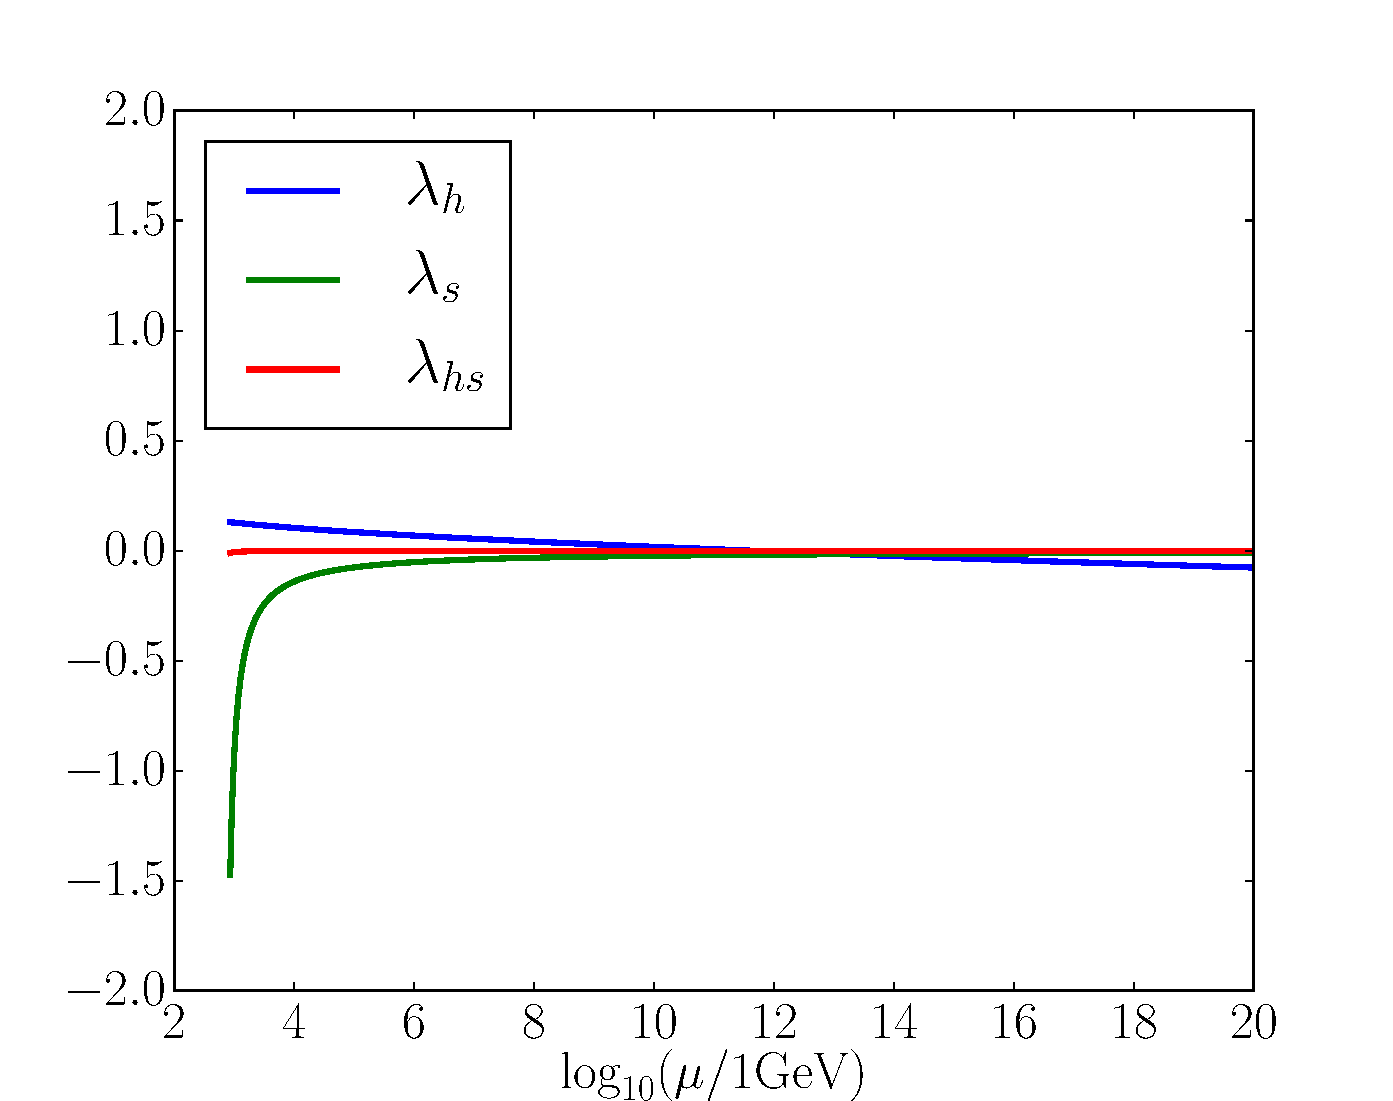
\includegraphics[width=\columnwidth]{scenario1}
\caption{Renormalization Group Flow of the coupling constants with $m_\sigma = \SI{3}{\tera\electronvolt}$ and $N_S=100$.}\label{fig:sce1}
\end{figure}

In order to solve the RG equations, we use the SM value of $\lambda_h$ at $\mu = m_\phi$, and \textsc{Eqs.}\ \eqref{eq:lhs} and \eqref{eq:ls} at $\mu=v_s$. Special care must be taken to make sure that the coupling constants remain in the perturbative regime ( i. e. $|\lambda| \leq 3$). Two different scenarios for $\lambda_s$ and $\lambda_{hs}$ are possible:
\begin{itemize}
\item In the limit $|\lambda_s|\to 0$,
\begin{equation}
\lambda_{hs} = -\sqrt{32\pi^2 \lambda_s}\ ,
\end{equation}
\begin{equation}
m_\sigma = 2 m_\phi \left(\frac{\lambda_s}{32\pi^2}\right)^{1/4}\ .
\end{equation}
The perturbativity of $\lambda_{hs}$ requires $|\lambda_s| < 0.03$, therefore $m_\sigma < 0.17 m_\phi$. This scenario is completely independent of the value of $N_s$.

\item When $|\lambda_s|$ approaches its maximum value allowed by \eqref{eq:lim_ls},
\begin{equation}
|\lambda_s| = \frac{16\pi^2}{4+N_S} - \delta \ \ \mathrm{as}\ \ \delta\to 0\ ,
\end{equation}
the other parameters are
\begin{equation}
\lambda_{hs} = -\sqrt{32\pi^2 \delta}\ ,
\end{equation}
\begin{equation}
m_\sigma = 2 m_\phi \frac{1}{\sqrt{N_S + 4 }}\left(\frac{8\pi^2}{\delta}\right)^{1/4}\ .
\end{equation}

In this case we need $N_s \geq 50$ if we insist on $|\lambda_s| \leq 3$. The mass of the scalar $S$ may grow as large as desired.
\end{itemize}

\begin{figure}[t]
\centering
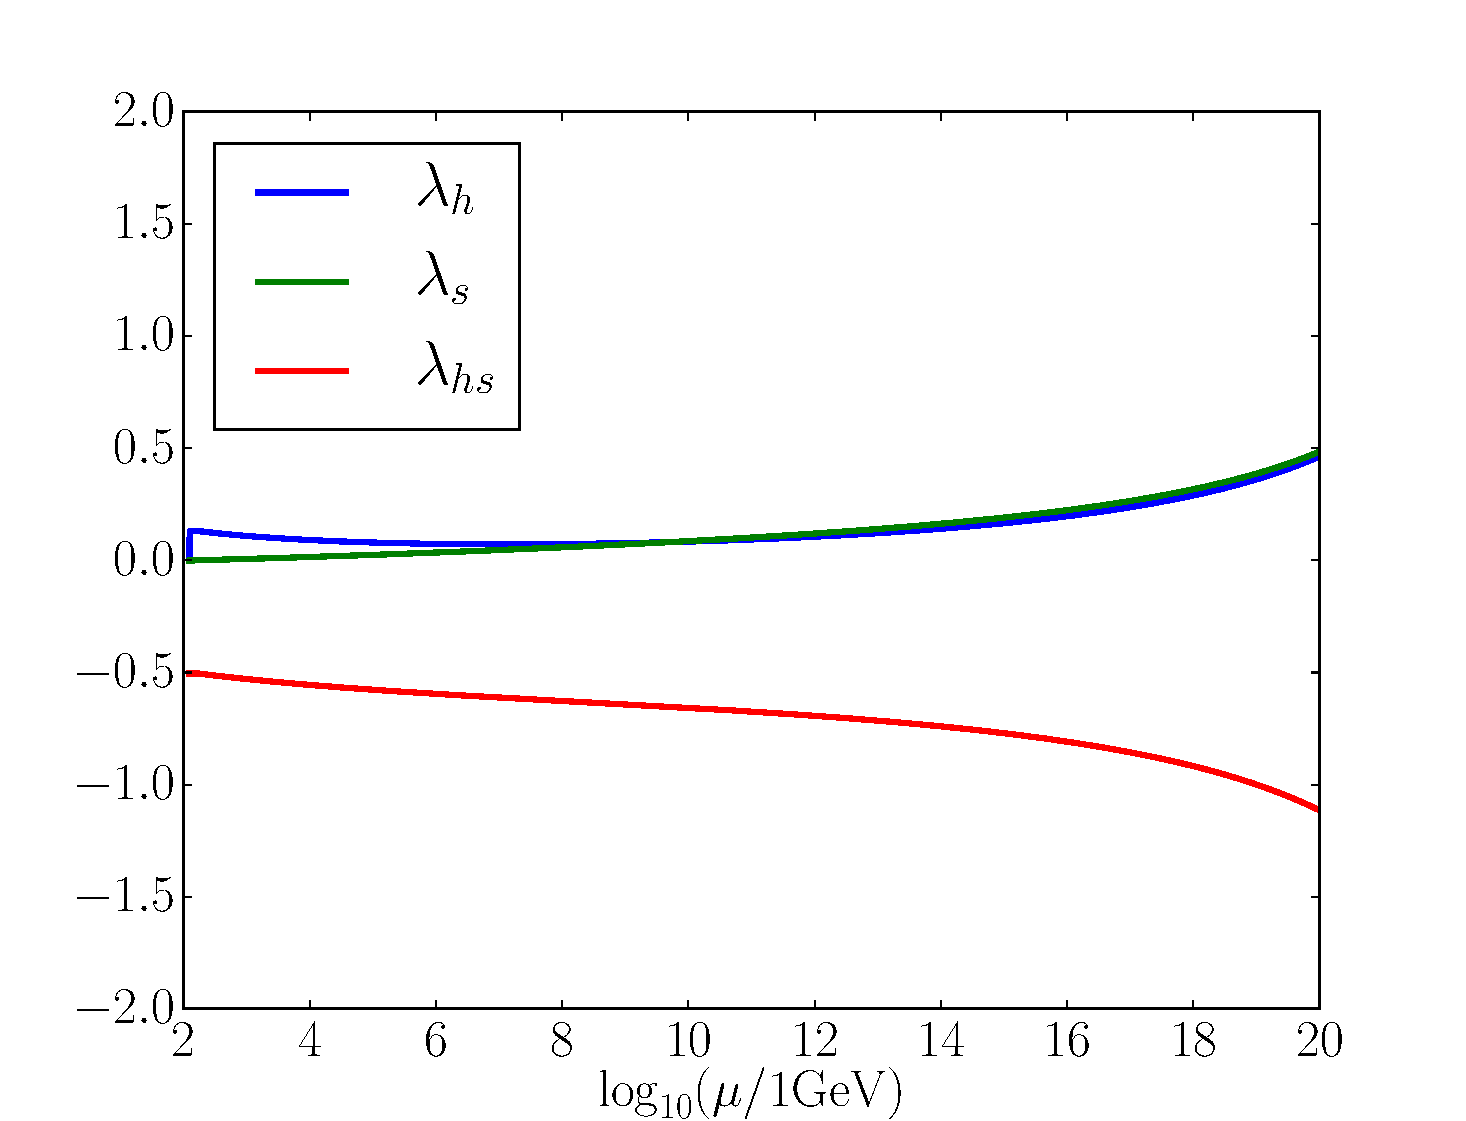
\includegraphics[width=\columnwidth]{scenario2}
\caption{Renormalization Group Flow of the coupling constants with $m_\sigma = \SI{10}{\giga\electronvolt}$ and $N_S=2$.}\label{fig:sce2}
\end{figure}

As an example of the second scenario, in \textsc{FIG.}\ref{fig:sce1} we show the behaviour of the coupling constants when $m_\sigma = \SI{3}{\tera\electronvolt}$ and $N_S = 100$. This set-up presents the nice feature that the three couplings meet at zero around the GUT scale. 



On the other hand, in the first scenario, the absolute value of the coupling constants grows with the energy until they reach a Landau pole at low energy. To retain the perturbativity until the Planck scale, the mass of the new scalar must be extremely low. In \textsc{Fig.} \ref{fig:sce2} we show the running of the couplings when $m_\sigma =\SI{10}{\giga\electronvolt}$ and $N_S = 2$. In this case, the unification of the constants at high energies is no longer possible. 




We also tried adding the new $\mathsf{SU}(N_S)$ symmetry group as a gauge group with its own dynamics, and with a coupling $g_4\neq 0$. When $g_4$ is small, of order $g_4\sim 0.1$, the Renormalization Group Equations dont't change qualitatively. But in the case $g_4 \gg 0.1$, the perturbativity of the theory breaks down at low energies. Therefore, we have decided not to consider non-zero values of $g_4$ at all.

\section{Mixing of the fields} \label{sec:mixing}
\begin{figure}[t]
\centering
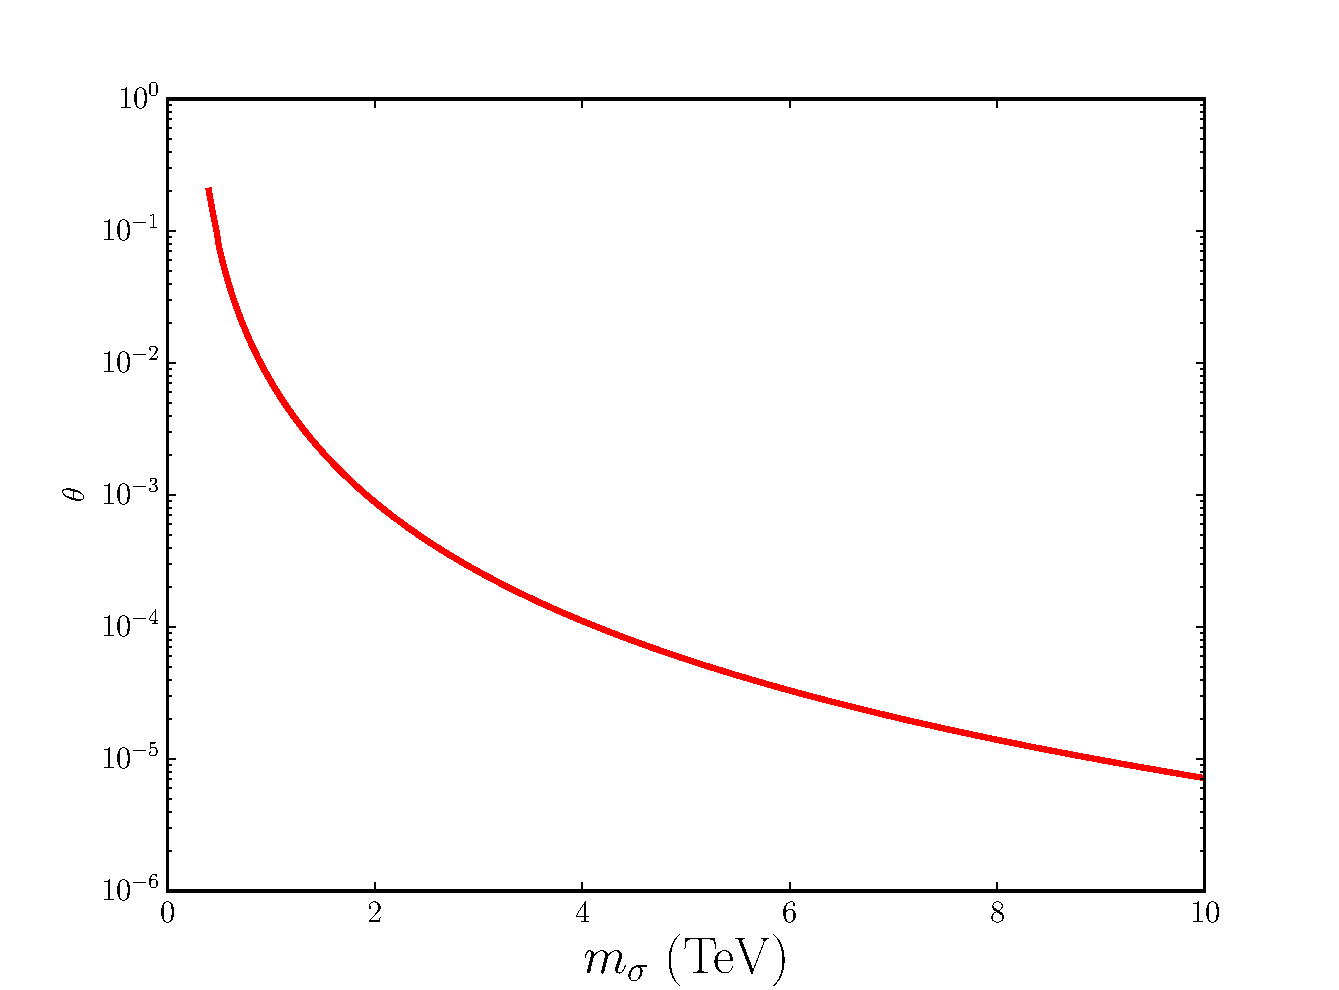
\includegraphics[width=\columnwidth]{angle}
\caption{Scalar mixing angle $\theta$ as a function of the mass $m_\sigma$ of the \textit{unmixed} field $S$. The value of $N_S$ is set to $N_S=150$.}\label{fig:angle}
\end{figure}

When both of the symmetries are broken, the $\phi$ and $\sigma$ fields are no longer mass eigenstates, since there is a quadratic term in the interaction potential that mixes them. The observable fields in this regime will be a combination of $\phi$ and $\sigma$, with different values for the masses. Before the breaking of the $\mathsf{SU}(2)$ group, the different symmetry protects the fields from mixing.

The quadratic term in the potential can be written as a quadratic form $V_q = \frac{1}{2}\Phi^\dagger \mathbb{M}^2 \Phi$, where $\Phi^\dagger = \begin{pmatrix}\phi & \sigma \end{pmatrix} $. The fields after the mixing will be the eigenstates of $\mathbb{M}^2$, and their squared masses are given by the eigenvalues of $\mathbb{M}^2$.

The quadratic part of the potential in the completely broken phase is
\begin{align}
V_q =& \frac{1}{2} m_\phi^2 \phi^2  + \frac{1}{2} m_\sigma^2 \sigma^2 + \frac{v_h}{\sqrt{2}} \left((2\lambda_{hs} + \beta_{hs})v_s + \beta_h \frac{v_h^2}{v_s} \right) \phi \sigma \nonumber\\
=& \frac{1}{2} \Phi^\dagger \begin{pmatrix} m_\phi^2 & m_{\phi\sigma}^2\\ m_{\phi\sigma}^2  & m_\sigma^2 \end{pmatrix}\Phi\ ,
\end{align}
where
\begin{equation}
m_{\phi\sigma}^2 = \frac{v_h}{\sqrt{2}} \left((2\lambda_{hs} + \beta_{hs})v_s + \beta_h \frac{v_h^2}{v_s} \right)\ .
\end{equation} 



The ``physical'' fields $(h, s)$ are given by a rotation of the $(\phi, \sigma)$ fields 
\begin{equation}
h = \phi \cos \theta - \sigma \sin \theta \qquad s = \phi \sin \theta + \sigma \cos \theta\ ,
\end{equation}
by the scalar mixing angle 
\begin{equation}
\theta = \frac{1}{2} \tan^{-1} \frac{2m_{\phi\sigma}^2}{m_\sigma^2 - m_\phi^2}\ .
\end{equation}

The masses of the physical fields are
\begin{align}
m_h^2 = m_\phi^2 \cos^2 \theta + m_\sigma^2 \sin^2 \theta - 2 m_{\phi\sigma}^2 \sin \theta \cos \theta\ , \\
m_s^2 = m_\sigma^2 \cos^2 \theta + m_\phi^2 \sin^2 \theta + 2 m_{\phi\sigma}^2 \sin \theta \cos \theta\ .
\end{align}

In the second scenario ($m_\sigma \gg m_h$, $N_S \geq 50$, $g_4=0$), the scalar mixing angle is found to be small, as is depicted in \textsc{fig.} \ref{fig:angle}. As the difference between the mass terms $m_\phi$ and $m_\sigma$ grows larger, the scalar mixing angle decreases rapidly. When $m_\sigma > \SI{2}{\tera\electronvolt}$, the scalar mixing angle is $\theta < \num{e-3}$. Thus, identifying $\phi$ as the ``true'' Higgs boson and $\sigma$ as another scalar particle is a very precise approximation. 

In the first scenario we find that the stationary point of the potential is in fact a saddle point, as the matrix $\mathcal{M}^2$ is not positive definite. Therefore, this solution is ruled out.


\section{Unification of the constants}\label{sec:GUT}

A common feature of most of the Beyond Standard Model theories is that they predict some sort of unification of the coupling constants at large energies, at the so-called Grand Unification Theory (GUT) scale. In \textsc{Fig.}\ref{fig:sce1} we have glimpsed that this might be the case in our model. In this section we will study this situation in more detail.

In order to quantify if the three quartic couplings are unified at a certain energy scale, we will define an \textit{unification distance} $d$ as
\begin{equation}
d = \frac{1}{3}(|\lambda_h - \lambda_s| + |\lambda_h - \lambda_{hs}|+ |\lambda_s - \lambda_{hs}|)\ .
\end{equation}

Obviously, a perfect unification of the three constants happens if and only if $d=0$.

\begin{figure}[t]
\centering
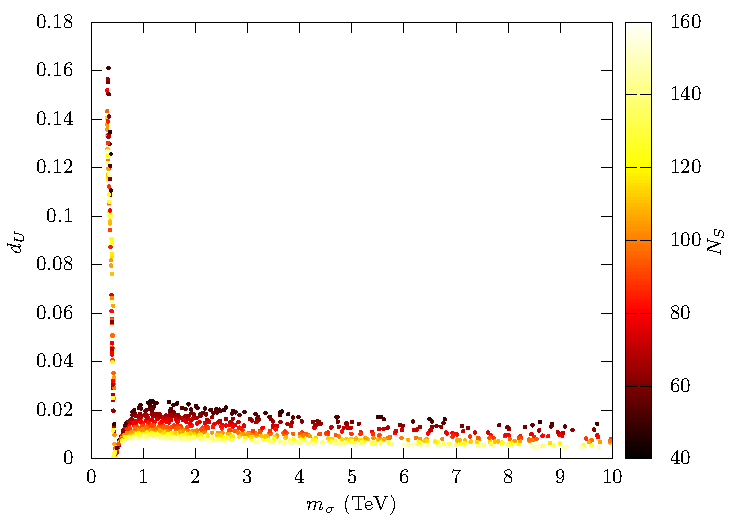
\includegraphics[width=\columnwidth]{GUTdistance}
\caption{Unification distance as a function of the mass $m_\sigma$ (horizontal axis) and $N_S$ (color code).}\label{fig:GUTdistance}
\end{figure}
\begin{figure}[t]
\centering
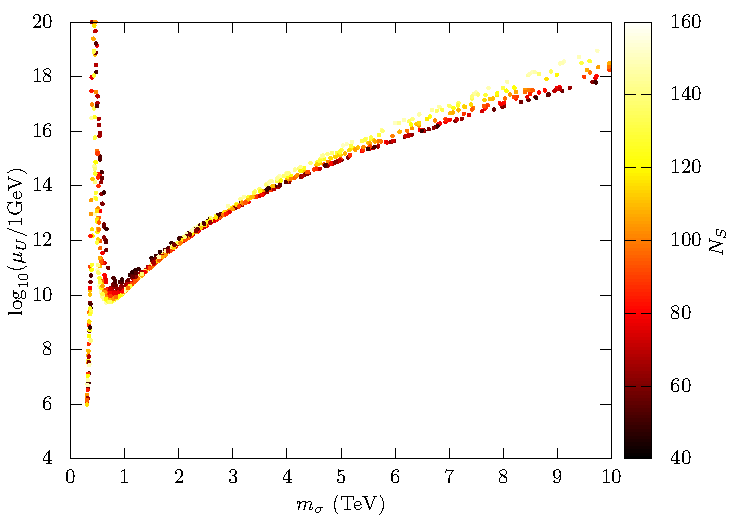
\includegraphics[width=\columnwidth]{GUTscale}
\caption{Unification scale as a function of the mass $m_\sigma$ (horizontal axis) and $N_S$ (color code).}\label{fig:GUTscale}
\end{figure}

We will pick a large sample of points in the $(m_\sigma, N_S)$ space of parameters to examine the unification of the couplings. The samples are chosen randomly with $N_S \leq 250$ and $m_\sigma \leq \SI{10}{\tera\electronvolt}$, and only those that preserve the perturbativaty up to the Planck scale are preserved. The final set consists of one thousand samples.

For each pair of parameters $(m_\sigma, N_S)$ we determine the minimum of the unification scale, $d_U$, and the energy scale which the minimum is attained at, $\mu_U$.  In \textsc{fig.} \ref{fig:GUTdistance} and \textsc{fig.} \ref{fig:GUTscale} we show the unification distance and scale as a function of $m_\sigma$. We find that both $d_U$ and $\mu_U$ depend largely on $m_\sigma$, and only exhibit a small dependence on $N_S$.


When the mass $m_\sigma$ is smaller than \SI{400}{\giga\electronvolt} the unification happens at energies above the Planck scale, so we can't speak of a true unification. With higher masses the unification scale remains small, of order $d_U \sim 0.01$, and the unification scale grows with the mass. To match the Grand Unification Theory scale, $\mu_{\mathrm{GUT}}\approx \SI{e15}{\giga\electronvolt}$, the scalar should have a mass between \SI{4}{\tera\electronvolt} and \SI{8}{\tera\electronvolt}. At a fixed value of $m_\sigma$, a larger value of $N_S$ means a better unification (i.e. a lower unification distance) and a slightly larger unification scale. 

\section{Phenomenology of the model}
In this model we have added a multiplet of $N_S$ scalar fields to the SM model. Initially, they only interact with the Higgs field via the $\lambda_{hs}$ coupling.

Nevertheless, after the symmetry breaking, one of the scalar fields gains a mass, and what is more important, mixes with the Higgs boson. Due to this mixing, the scalar $s$ is able to decay in the same channels that the Higgs (fermion-antifermion, WW, ZZ,  gluon-gluon, $\gamma\gamma$, Z$\gamma$), but the amplitudes are suppressed by a factor $\sin \theta$, and the cross-sections and decay widths by a factor $\sin^2\theta$. 

The coupling between one scalar $s$ and two Higgs bosons $h$ arises from the interaction potential \eqref{eq:interlagr} and the cubic term in \eqref{eq:Spotential}. After performing the spontaneous breaking of $H$ into $\phi$ and the mixing of $\phi$ and $\sigma$, this interaction is
\begin{equation}
\mathcal{L}_{hhs} = \frac{\kappa}{2} h^2 s\ ,
\end{equation}
where
{\scriptsize\begin{align}
\kappa =& \left(\frac{(2\lambda_{hs} + \beta_{hs})v_s}{\sqrt{2}} + 6 v_h^2\frac{\beta_h}{\sqrt{2} v_s} \right)\cos^3 \theta \nonumber\\
&+ \left(-4\sqrt{2}v_h \frac{2\lambda_{hs} + 3\beta_{hs}}{4} - 8\sqrt{2}v_h^3  \frac{\beta_h}{4 v_s^2} \right)\cos^2\theta \sin \theta \nonumber\\
&+ \left(-2\frac{(2\lambda_{hs} + \beta_{hs})v_s}{\sqrt{2}} -12 v_h^2\frac{\beta_h}{\sqrt{2} v_s} +6\sqrt{2}(\lambda_s+\beta_s) v_s \right)\cos\theta \sin^2\theta \nonumber\\
&+\left(2\sqrt{2}v_h \frac{2\lambda_{hs} + 3\beta_{hs}}{4} -4\sqrt{2}v_h^3 \frac{\beta_h}{4 v_s^2} \right)\sin^3\theta\ .
\end{align}}

The decay amplitude for this process is simply
\begin{equation}
\mathcal{M}(s\to hh)= -i \kappa\ ,
\end{equation}
and the decay width, using the well-known phase space for two identical particles, is
\begin{equation}
\Gamma(s\to hh) = \frac{|\mathcal{M}|^2}{8\pi m_s}\sqrt{1-\frac{4m_h^2}{m_s^2}} = \frac{\kappa^2}{8\pi m_s}\sqrt{1-\frac{4m_h^2}{m_s^2}}\ .
\end{equation}

The interaction between the top quark and $s$ comes from the Yukawa coupling 
\begin{equation}
\mathcal{L}_t = -\frac{m_t}{v_h}\bar{t}\phi t=  -\frac{m_t}{v_h}\sin\theta\, \bar{t} s t-\frac{m_t}{v_h}\cos\theta\, \bar{t} h t\ ,
\end{equation}
so the squared amplitude decay is 
\begin{align}
|\mathcal{M}(s\to t\bar{t})|^2 =& N_c \frac{m_t^2}{v_h^2}\sin^2\theta \tr[(\sla{p_1} + m_t)(\sla{p_2}-m_t)]\nonumber\\
=& N_c \frac{2 m_t^2 m_s^2 }{v_h^2} \sin^2 \theta \left(1-\frac{4 m_t^2}{m_s^2}\right)\ ,
\end{align}
and the resulting decay width is
\begin{equation}
\Gamma(s \to t \bar{t})= \frac{3 m_t^2 m_s \sin^2\theta}{8\pi  v_h^2} \left(1-\frac{4 m_t^2}{m_s^2}\right)^{3/2} \ ,
\end{equation}

In the same fashion, the interaction with the $W$ and $Z$ bosons  arises from
\begin{align}
\mathcal{L}_W =& 2 \frac{m_W^2}{v_h}\phi W^+_\mu W^{-\mu} + \frac{m_Z^2}{v_h} \phi Z_\mu Z^\mu\nonumber\\
=& 2 \sin \theta \frac{m_W^2}{v_h}s W^+_\mu W^{-\mu} + \sin\theta \frac{m_Z^2}{v_h} s Z_\mu Z^\mu + \cdots
\end{align}
so the squared amplitude decay to $WW$ is
\begin{align}
|\mathcal{M}(s\to W^+W^-)|^2 =& \frac{4 m_W^4 \sin^2\theta}{v_h^2} \left(-g^{\mu\nu}+\frac{p^\mu_1 p^\nu_2}{m_W^2} \right)^2\nonumber\\
=&  \frac{m_W^4 \sin^2 }{m_s v_h^2} \left(3+\frac{m_s^4}{4 m_W^4}-\frac{m_s^2}{m_W^2} \right)\ ,
\end{align}
and the decay width results
\begin{equation}
\Gamma(s \rightarrow WW)=  \frac{\sin^2\theta }{4 \pi } \frac{m_W^4}{m_s v_h^2} \sqrt{ 1- \frac{4 m_W^2}{m_s^2}}
\left(3+\frac{m_s^4}{4 m_W^4}-\frac{m_s^2}{m_W^2} \right)\ .
\end{equation}

The decay width to $ZZ$ displays an extra $1/2$ factor due to the symmetry of identical paricles:
\begin{equation}
\Gamma(s \rightarrow ZZ)=  \frac{\sin^2\theta }{8 \pi } \frac{m_Z^4}{m_s v_h^2} \sqrt{ 1- \frac{4 m_Z^2}{m_s^2}}
\left(3+\frac{m_s^4}{4 m_Z^4}-\frac{m_s^2}{m_Z^2} \right)\ .
\end{equation}

\begin{figure}[t]
\centering
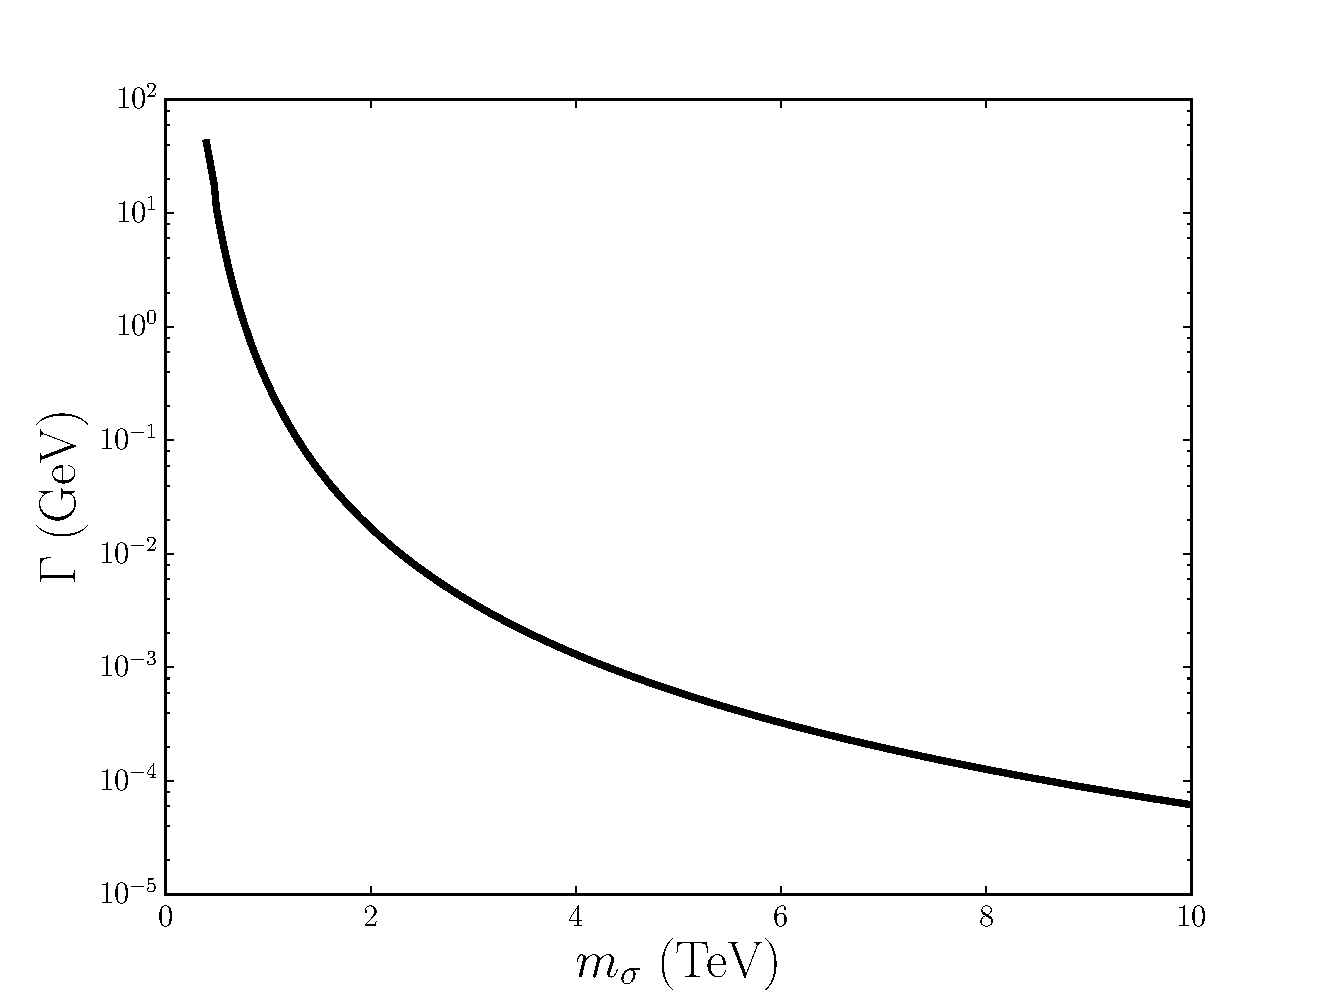
\includegraphics[width=\columnwidth]{totalwidth}
\caption{Total decay width (considering $hh$, $t\bar{t}$, $WW$ and $ZZ$ channels) of the scalar $s$.}\label{fig:totalwidth}
\end{figure}
\begin{figure}[t]
\centering
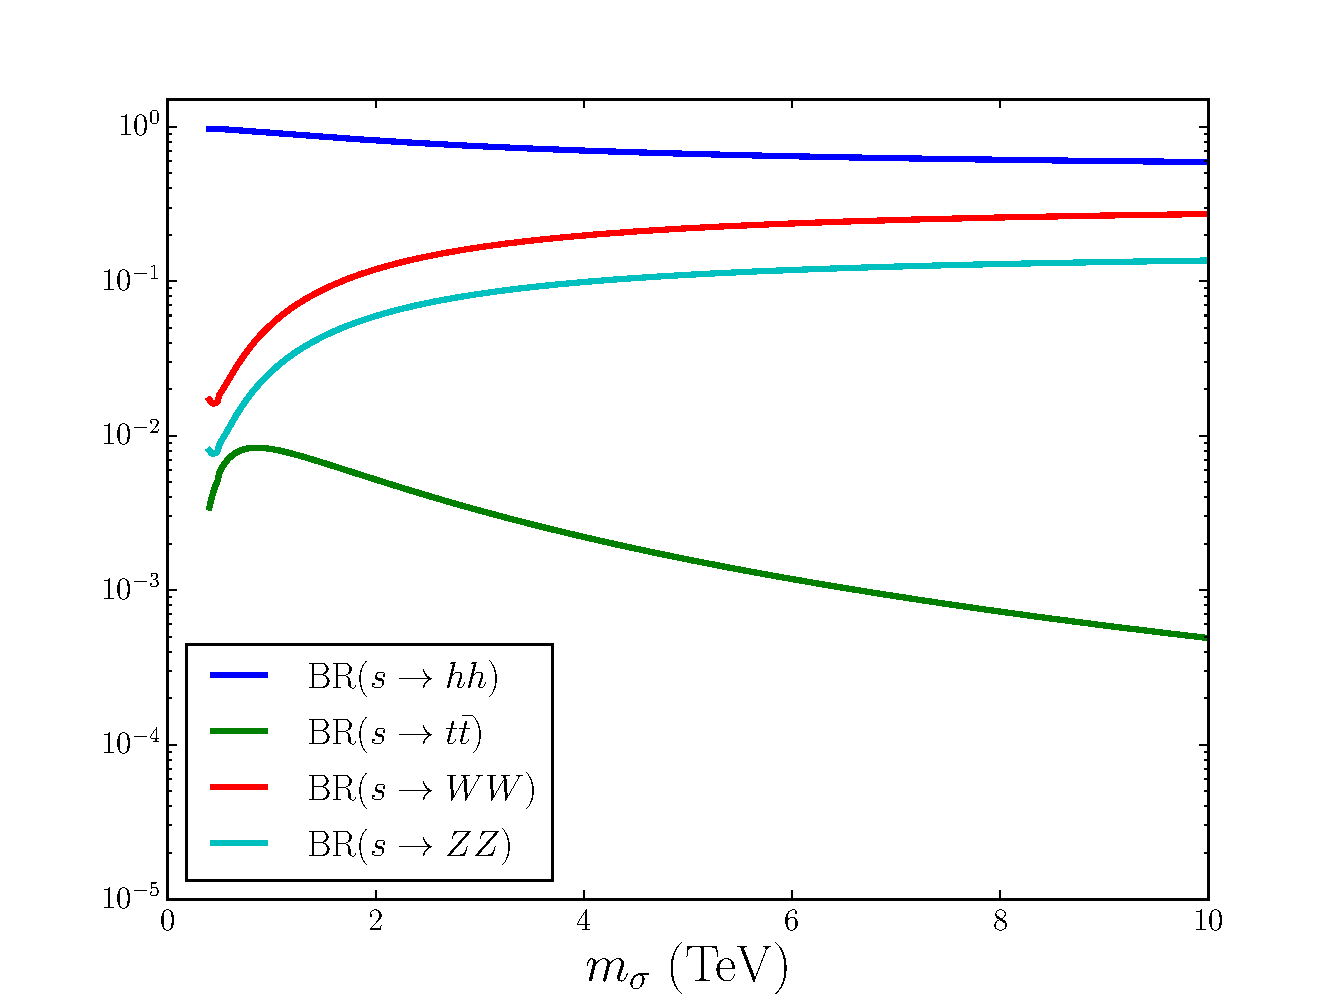
\includegraphics[width=\columnwidth]{BR}
\caption{Branching ratios for the decay of $s$ in the $hh$, $t\bar{t}$, $WW$ and $ZZ$ channels.}\label{fig:BR}
\end{figure}

In \textsc{fig.} \ref{fig:totalwidth} is shown the total decay width of the scalar $s$, and in \textsc{fig.} \ref{fig:BR} the branching ratios for the main decay channels. The decay to two Higgs bosons is the dominant channel, since the Higgs-like decays are suppressed by a factor $\sin^2\theta$.


\bibliographystyle{apsrev4-1}
\bibliography{memoria} 

\newpage
\clearpage

\begin{widetext}
El abajo firmante, matriculado en el Máster de Física Teórica de la Facultad de Ciencias Físicas, autoriza a la Universidad Complutense de Madrid (UCM) a difundir y utilizar con fines académicos, no comerciales y mencionando expresamente a su autor el presente Trabajo de Fin de Máster: Nuevas aplicaciones del modelo de Coleman-Weinberg, realizado durante el curso académico 2015-2016 bajo la dirección de Jose A. Ruiz Cembranos en el Departamento de Física Teórica I, y a la Biblioteca de la UCM a depositarla en el Archivo institucional E-Prints Complutense u otra plataforma de la UCM que se cree para tal fin con el objeto de incrementar la difusión, uso e impacto del trabajo en Internet y garantizar su preservación y acceso a largo plazo.\\

La publicación en abierto tendrá un embargo de:
\\

\noindent$\,X\,$ Ninguno
\\


Fdo:\\


\vspace{3cm}

El abajo firmante, director del Máster de Física Teórica de la Facultad de Ciencias Físicas, autoriza a la Universidad Complutense de Madrid (UCM) a difundir y utilizar con fines académicos, no comerciales y mencionando expresamente a su autor el presente Trabajo de Fin de Máster: Nuevas aplicaciones del modelo de Coleman-Weinberg, realizado durante el curso académico 2015-2016 bajo mi dirección en el Departamento de Física Teórica I, y a la Biblioteca de la UCM a depositarla en el Archivo institucional E-Prints Complutense u otra plataforma de la UCM que se cree para tal fin con el objeto de incrementar la difusión, uso e impacto del trabajo en Internet y garantizar su preservación y acceso a largo plazo.\\

La publicación en abierto tendrá un embargo de:
\\

\noindent$\,X\,$ Ninguno
\\


Fdo:\\


\vspace{12cm}

\end{widetext}



\end{document} 
